\begin{figure}[htbp]
\centering
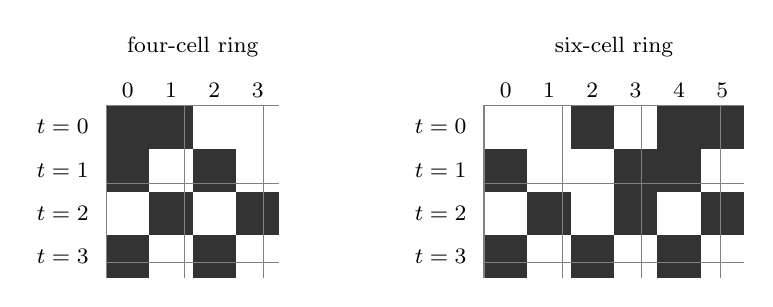
\begin{tikzpicture}[x=0.55cm,y=0.55cm,font=\footnotesize]
  \node at (2,1.35) {four-cell ring};
  \foreach \x in {0,1,2,3} \node at (\x+0.5,0.35) {$\x$};
  \foreach \t in {0,1,2,3} \node[left] at (-0.18,-\t-0.5) {$t=\t$};
  \foreach \x/\t in {0/0,1/0,0/1,2/1,1/2,3/2,0/3,2/3}
    \fill[black!80] (\x,-\t) rectangle ++(1,-1);
  \draw[gray] (0,0) grid (4,-4);
  \begin{scope}[xshift=4.8cm]
    \node at (3,1.35) {six-cell ring};
    \foreach \x in {0,1,2,3,4,5} \node at (\x+0.5,0.35) {$\x$};
    \foreach \t in {0,1,2,3} \node[left] at (-0.18,-\t-0.5) {$t=\t$};
    \foreach \x/\t in {2/0,4/0,5/0,0/1,3/1,4/1,1/2,3/2,5/2,0/3,2/3,4/3}
      \fill[black!80] (\x,-\t) rectangle ++(1,-1);
    \draw[gray] (0,0) grid (6,-4);
  \end{scope}
\end{tikzpicture}
\caption{Rule-184 updates on two rings, with time downward, cell indices increasing to the right, and occupied cells filled. The rightmost cell is adjacent to cell $0$ in each ring.}
\label{fig:rule184}
\end{figure}
